\chapter{Appendix}
\section{Lagrangian physics}

\begin{center}
\includegraphics[scale=0.4]{continuum_mapping.png}
\end{center}
Let $ \hat{\mathcal{S}}$, $\mathcal{S}$, $\mathcal{S}(t)$ be the initial stress free configuration of a given body, the reference and the current configuration respectively.
I define a smooth mapping from the reference configuration to the current configuration:
\begin{equation}
\chi^s(\textbf{X},t) : \hat{\mathcal{S}} \rightarrow \mathcal{S}(t)     
\end{equation}
Where $\textbf{X}$ denotes a material point in the reference domain and $\chi^s$ denotes the mapping from the reference configuration to the current configuration. Let $d^s(\textbf{X},t)$ denote the displacement field which describes deformation on a body. The mapping $\chi^s$ can then be specified from a current position plus the displacement from that position:
\begin{equation} \label{eq:chi}
 \chi^s(\textbf{X},t) = \textbf{X}  + d^s(\textbf{X} ,t) 
\end{equation}
which can be written in terms of the displacement field:
\begin{equation}
 d^s(\textbf{X},t) = \chi^s(\textbf{X},t) -\textbf{X}   
\end{equation}

Let w(\textbf{X},t) be the domain velocity which is the partial time derivative of the displacement: 
\begin{equation}
 w(\textbf{X},t) = \frac{\partial \chi^s(\textbf{X},t)}{\partial t}   
\end{equation}

\subsection{Deformation gradient}
The deformation gradient describes the rate at which a bode undergoes deformation.
Let $d(\textbf{X},t)$ be a differentiable deformation field in a given body, the deformation gradient is then:  
\begin{equation}
\label{eq:deformation_gradient}
F = \frac{\partial \chi^s(\textbf{X},t)}{\partial \textbf{X}} = \frac{\partial \textbf{X}  + d^s(\textbf{X} ,t) }{\partial \textbf{X}} =  I + \nabla d(\textbf{X},t) 
\end{equation}
which denotes relative change of position under deformation in a Lagrangian frame of reference. We can observe that when there is no deformation. The deformation gradient $F$ is simply the identity matrix. \newline

Let the Jacobian determinant, which is the determinant of the of the deformation gradient F, be defined as:
\begin{equation}\label{eq:J}
J = \text{det}(F)
\end{equation}
The Jacobian determinant is used to change between volumes, assuming infinitesimal line and area elements in the current $ds, dx$ and reference $dV,dX$ configurations. The Jacobian determinant is therefore known as a volume ratio.

\begin{comment}
The volume elements $dv, dV$ can be expressed by the dot product:
\begin{equation}
 dv = ds\cdot dx = J dS dX
\end{equation}
This is used to get the Nansons formula:
\begin{equation}\label{eq:Nanson}
ds = JF^{-T}dS
\end{equation}
which holds for an arbitrary line element in different configurations. This will be useful later on when describing equations in different configurations.
\end{comment}

\subsection{Strain}
\begin{figure}[H]
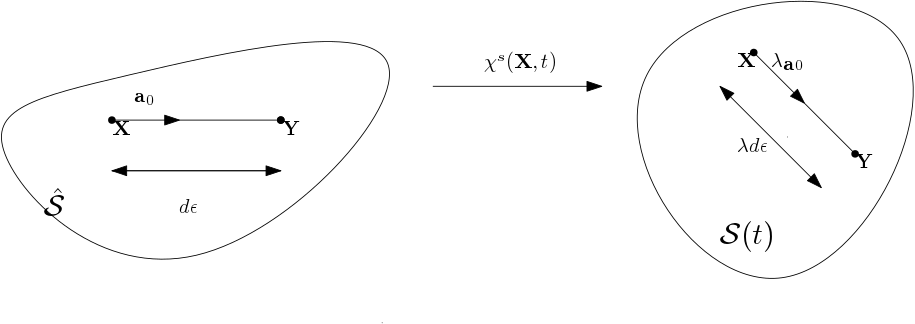
\includegraphics[scale=0.40]{./Solid_equations/Strain.png}
\caption{Deformation of a line element with length $d\epsilon$ into a line element with length $\lambda d \epsilon$}
\end{figure}


Strain is the relative change of location between two particles. Strain, strain rate and deformation is used to describe the relative motion of particles in a continuum. This is the fundamental quality that causes stress \cite{Richter2016}.

Observing two neighboring points \textbf{X} and \textbf{Y}. Let \textbf{Y} be described by adding and subtracting the point \textbf{X} and rewriting \textbf{Y} from the point \textbf{X} plus a distance $d\textbf{X}$   :
\begin{equation}
\textbf{Y} = \textbf{Y} + \textbf{X} - \textbf{X} = \textbf{X} + |\textbf{Y} - \textbf{X}| \frac{\textbf{Y} - \textbf{X}}{|\textbf{Y} - \textbf{X}|} = \textbf{X} + d\textbf{X}
\end{equation}

Let $d\textbf{X}$ be denoted by:
\begin{align}
d\textbf{X} =& d\epsilon \textbf{a}_0\\
d\epsilon =& |\textbf{Y} - \textbf{X}| \\
\textbf{a}_0 =& \frac{\textbf{Y} - \textbf{X}}{|\textbf{Y} - \textbf{X}|}
\end{align}
where $d\epsilon$ is the distance between the two points and $\textbf{a}_0$ is a unit vector 

We see now that $d\textbf{X}$ is the distance between the two points times the unit vector or direction from $\textbf{X}$ to $\textbf{Y}$.
\newline

A certain motion transform the points $\textbf{Y}$ and $\textbf{X}$ into the displaced positions $\textbf{x} = \chi^s(\textbf{X},t)$ and $\textbf{y} = \chi^s(\textbf{Y},t)$. Using Taylor?s expansion \textbf{y} can be expressed in terms of the deformation gradient:

\begin{align}
\textbf{y} =& \chi^s(\textbf{Y},t) = \chi^s(\textbf{X} + d\epsilon \textbf{a}_0,t) \\
=& \chi^s(\textbf{X},t) + d\epsilon F \textbf{a}_0 + \mathcal{O}(\textbf{Y}-\textbf{X}) 
\end{align}

where $\mathcal{O} (\textbf{Y}-\textbf{X})$ refers to the small error that tends to zero faster than $(\textbf{X} - \textbf{Y}) \rightarrow \mathcal{O}$. \newline

Setting $\textbf{x} = \chi^s(\textbf{X},t)$  It follows that:
\begin{align}
\textbf{y} - \textbf{x} =&  d\epsilon F \textbf{a}_0 + \mathcal{O}(\textbf{Y}-\textbf{X}) \\
=& F(\textbf{Y} - \textbf{X}) + \mathcal{O}(\textbf{Y}-\textbf{X}) 
\end{align}

Let the $\textbf{stretch vector}$ be $\lambda_{\textbf{a}0}$, which goes in the direction of $\textbf{a}_0$: 
\begin{equation}
\lambda_{\textbf{a}0}(\textbf{X},t) = F(\textbf{X},t)\textbf{a}_0 
\end{equation}

Looking at the square of $\lambda$:
\begin{align}
\lambda^2 &=  \lambda_{\textbf{a}0} \lambda_{\textbf{a}0} = F(\textbf{X},t)\textbf{a}_0 F(\textbf{X},t)\textbf{a}_0 \\
&= \textbf{a}_0 F^TF\textbf{a}_0 = \textbf{a}_0 C \textbf{a}_0
\end{align}

We have not introduced the important right Cauchy-Green tensor:
 \begin{equation}
 C = F^TF
\end{equation}
Since $\textbf{a}_0 $ is just a unit vector, we see that C measures the squared length of change under deformation. We see that in order to determine the stretch one needs only the direction of $\textbf{a}_0$ and the tensor C.
C is also symmetric and positive definite $C = C^T$.  I also introduce the Green-Lagrangian strain tensor E:
\begin{equation}\label{eq:StrainTensor}
E = \frac{1}{2}(F^TF -I) 
\end{equation}
which is also symmetric since C and I are symmetric. The Green-Lagrangian strain tensor E has the advantage of having no contributions when there is no deformations. Where the Cauchy-Green tensor gives the identity matrix for zero deformation.
		
\subsection{Stress}
While strain, deformation and strain rate only describe the relative motion of particles in a given volume, stress give us the internal forces between neighboring particles. Stress is responsible for deformation and is therefore crucial in continuum mechanics. The unit of stress is force per area.


that completely define the state of stress at a point inside a material in the deformed state, placement, or configuration. The tensor relates a unit-length direction vector n to the stress vector T(n) across an imaginary surface perpendicular to n:


Introducing the Cauchy stress tensor $\sigma_s$, which define the state of stress inside a material. The version of Cauchy stress tensor is defined by the material model used. 
If we use this tensor on an area, taking the stress tensor times the normal vector $\sigma_s \bold{n}$ we get the forces acting on that area.

Stress tensor defined from the Cauchy by the constitutive law of St. Venant-Kirchhoff hyperelastic material model: 
\begin{equation}
 \sigma_s = \frac{1}{J} F(\lambda_s (tr E)I + 2\mu_sE) F^T
\end{equation}

Using the deformation gradient and the Jacobian determinant., I get the first Piola-Kirchhoff stress tensor P:
\begin{equation}
 P = J \sigma F^{-T} 
\end{equation}
This is known as the \textit{Piola Transformation} and maps the tensor into a Lagrangian formulation which will be used when stating the solid equation.

Introducing the second Piola-Kirchhoff stress tensor S:
\begin{equation}
S = J F^{-1}\sigma F^{-T} = F^{-1} P = S^T 
\end{equation}
from this relation the first Piola-Kirchhoff tensor can be expressed by the second:
\begin{equation}
P = FS
\end{equation}


\section{Results}
\begin{figure}[H]
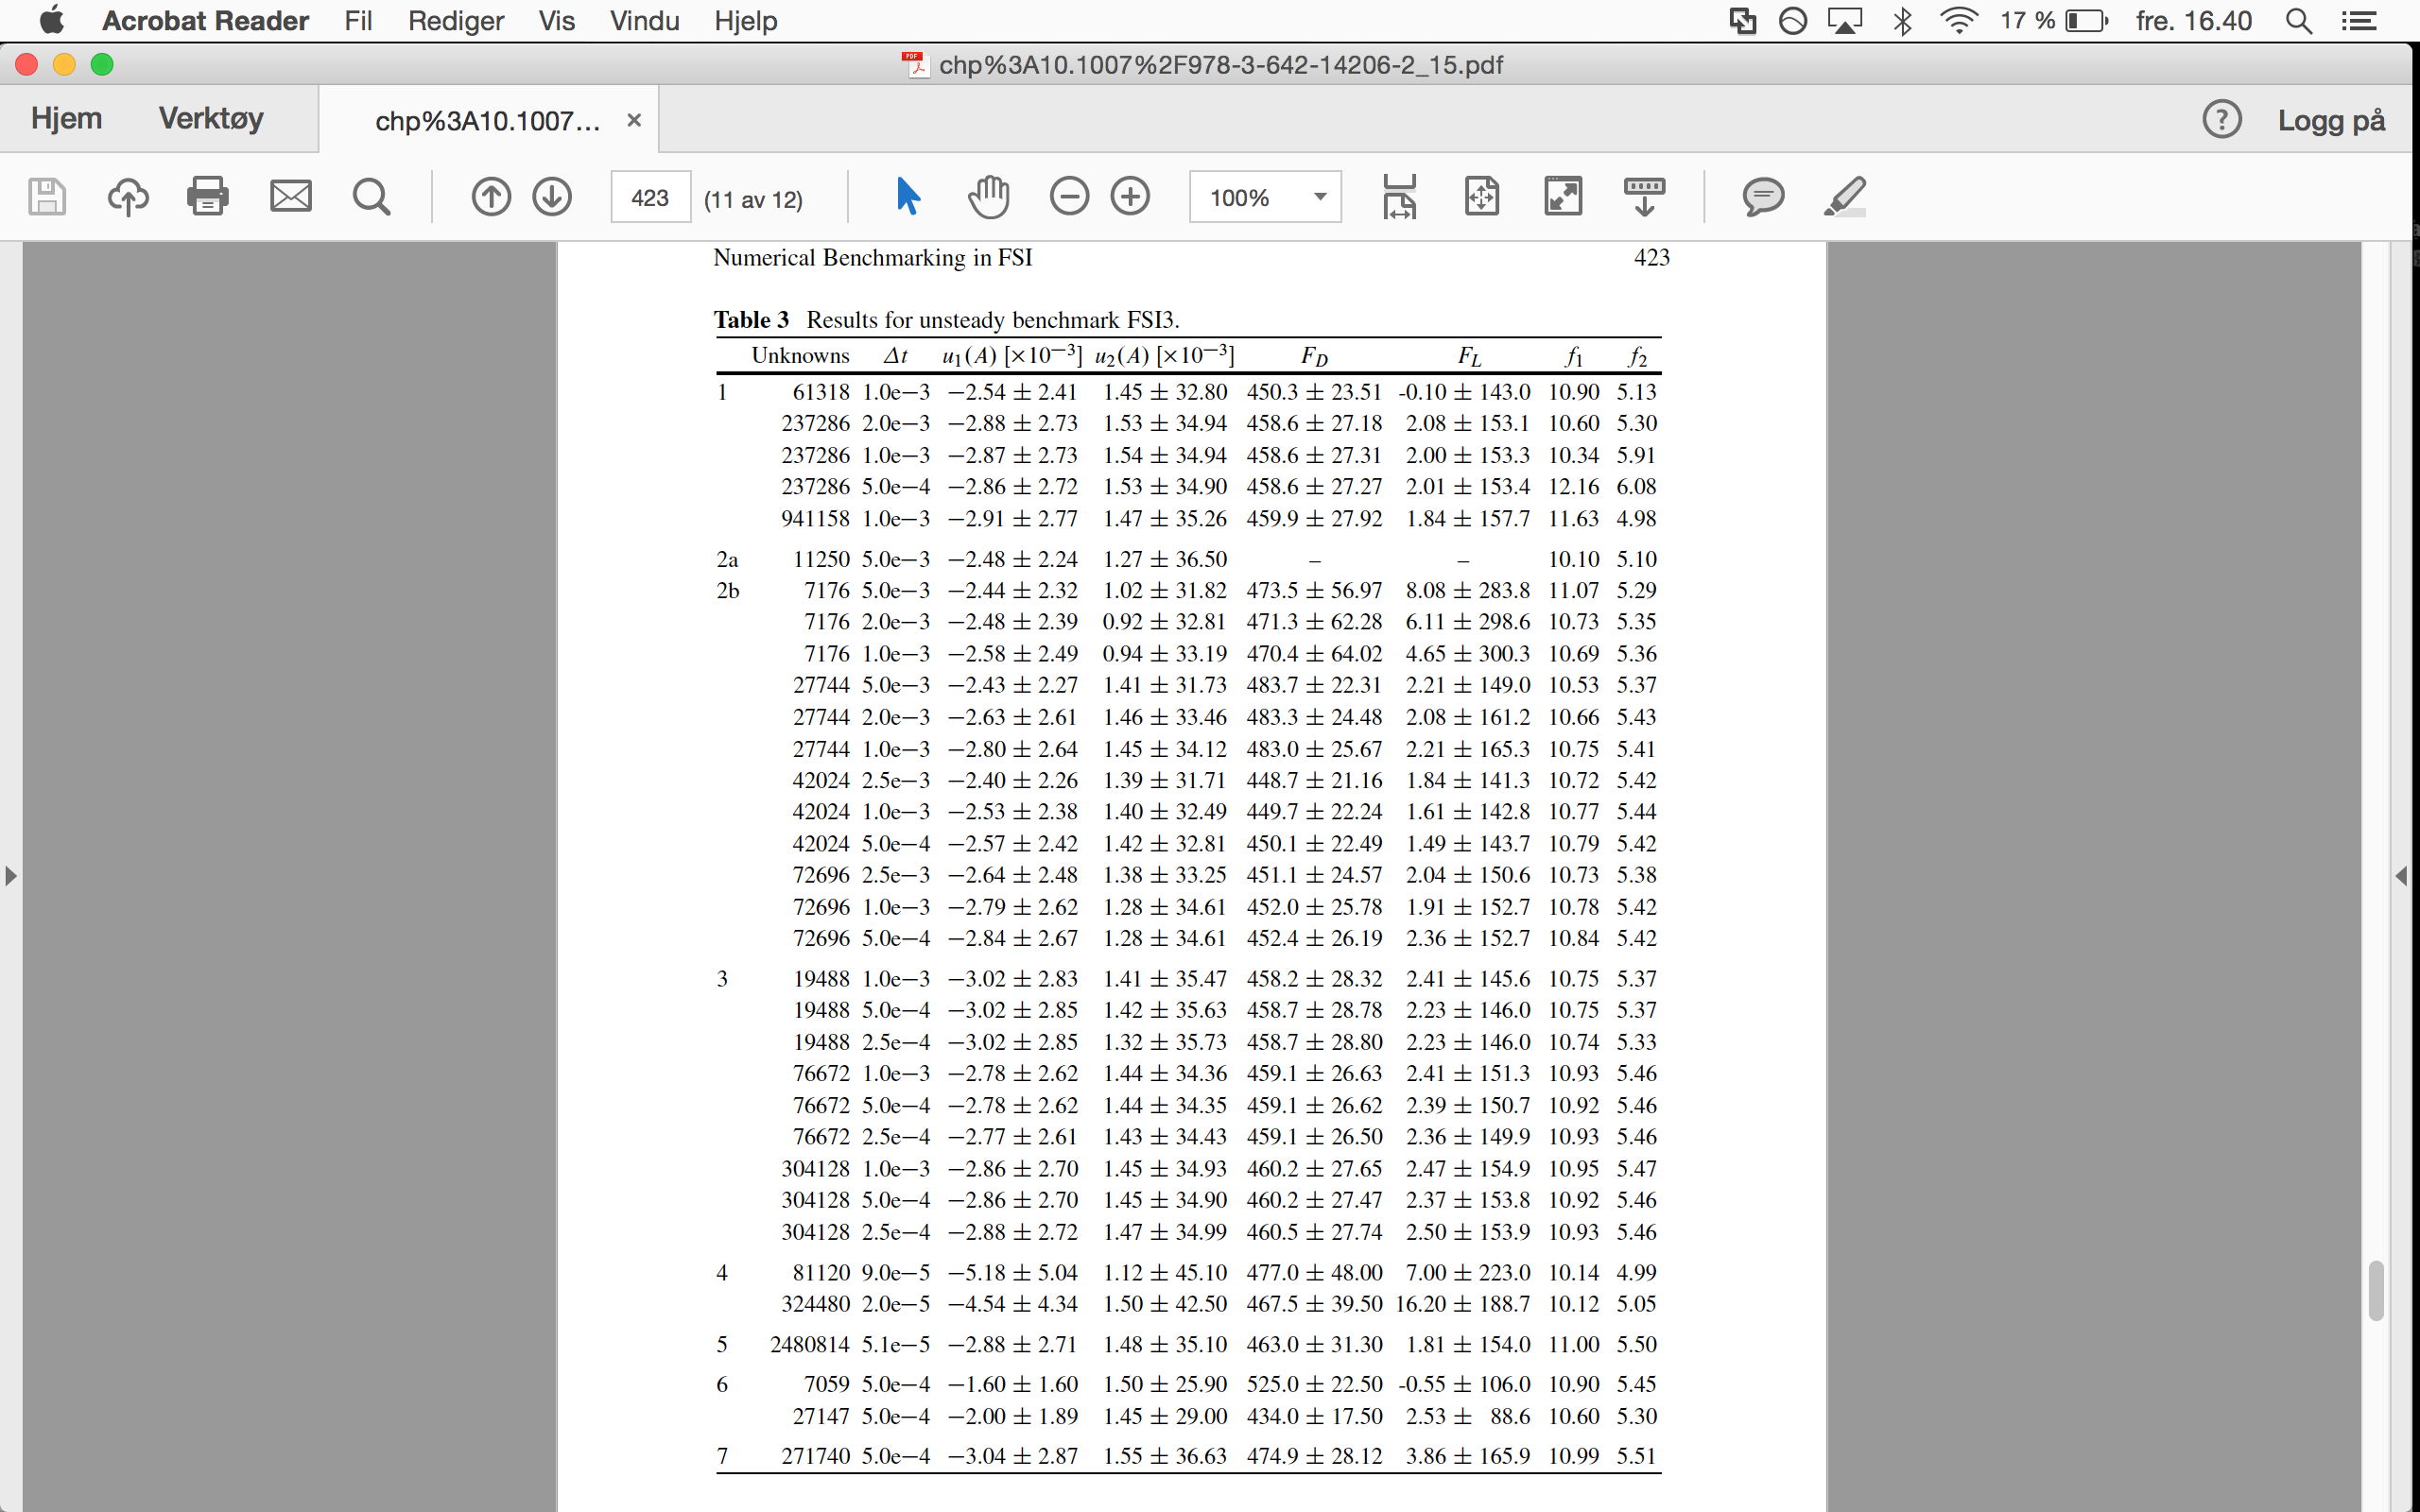
\includegraphics[scale=0.7,trim={12cm 0cm 16.3cm 5.5cm},clip]{./Appendix/BigBoyResults.png}
\caption{Results from different contributions in from the paper Turek et.al 2010 \cite{Turek2010}}
\end{figure}


\cite{Turek2010}



